\documentclass[10pt,a4paper]{article}
\usepackage[margin=1.8cm]{geometry}
\usepackage[T1]{fontenc}
\usepackage{lmodern}
\usepackage{microtype}
\usepackage{amsmath}
\usepackage{booktabs}
\usepackage{tabularx}
\usepackage{xcolor}
\usepackage{colortbl}
\usepackage{pgfplots}
\pgfplotsset{compat=1.18}
\usepackage[hyphens]{url}
\usepackage{hyperref}
\definecolor{served}{HTML}{DBEAFE}
\definecolor{bad}{HTML}{FEE2E2}
\definecolor{cfree}{HTML}{2563EB}
\hypersetup{colorlinks=true,linkcolor=cfree,urlcolor=cfree}
\newcolumntype{L}{>{\raggedright\arraybackslash}X}
\newcolumntype{C}{>{\centering\arraybackslash}X}

\title{\textbf{Decide: score against approach}\\[2pt]\large Every experiment and its measured score}
\author{Amal Verma}
\date{October 2026}

\begin{document}
\maketitle
\noindent All numbers were measured in this project with the judges' own scoring code
(\texttt{selfcheck.py}, or \texttt{offline\_score.py}, which reuses its metric functions).
Totals are out of 100. Weights: quality 40\%, calibration 25\%, latency 20\%, abstention 15\%.
Blue rows are the served configuration; red rows were rejected.

\section{Full self-check on the public dev split}
End-to-end runs through the real web service, int8 model on CPU.

\medskip
\noindent{\small
\begin{tabularx}{\linewidth}{@{}rLlccccccl@{}}
\toprule
\# & Approach & Trained on & Total & Qual. & Calib. & Lat. & Abst. & p95 & Verdict \\
\midrule
1 & Classical baseline: TF-IDF + LR, LightGBM + tabular & train & 78.45 & .783 & .760 & 1.00 & .542 & 22.5 & gate-1 baseline \\
2 & H384 + MoE, symmetric abstention & train & 83.76 & .850 & .856 & 1.00 & .558 & $\sim$24 & superseded \\
\rowcolor{served} 3 & \textbf{H384 + MoE, lopsided approve band} & \textbf{train} & \textbf{83.75} & .849 & .856 & 1.00 & .558 & \textbf{10.6} & \textbf{served} \\
4 & H768 NLI + MoE (quiet machine) & train & 84.52 & .846 & .849 & 1.00 & .632 & 21.3 & 2$\times$ slower; grounded p95 24.7 \\
5 & H768 NLI + MoE (busy machine) & train & 73.65 & .828 & .849 & 0.49 & .632 & 63 & latency risk \\
\rowcolor{bad} 6 & H384 + MoE retrained on train + dev & train+dev & 87.55 & .876 & .883 & 1.00 & .695 & 10.8 & rejected: inflated \\
\bottomrule
\end{tabularx}}

\medskip
\noindent p95 is the mean of the per-decision p95 latency in ms. The served model (\#3)
measured 78.26 on a busy machine (load 11): identical quality, calibration and abstention,
only latency dropped.

\begin{center}
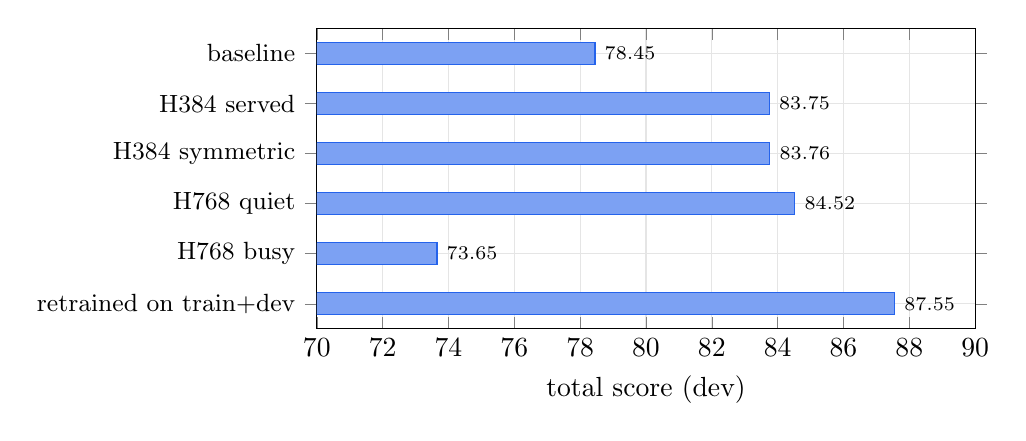
\begin{tikzpicture}
\begin{axis}[xbar, width=0.82\linewidth, height=5.4cm, xmin=70, xmax=90,
  symbolic y coords={{retrained on train+dev},{H768 busy},{H768 quiet},{H384 symmetric},{H384 served},{baseline}},
  ytick=data, y tick label style={font=\small}, xlabel={total score (dev)},
  nodes near coords, every node near coord/.append style={font=\scriptsize},
  bar width=8pt, grid=major, grid style={gray!20}]
\addplot[fill=cfree!60,draw=cfree] coordinates {(78.45,{baseline}) (83.75,{H384 served}) (83.76,{H384 symmetric}) (84.52,{H768 quiet}) (73.65,{H768 busy}) (87.55,{retrained on train+dev})};
\end{axis}
\end{tikzpicture}
\end{center}

\section{Offline score on dev (fp32, latency held at full marks)}
\begin{center}
\begin{tabular}{lcl}
\toprule
Approach & Total & Note \\
\midrule
H384 + MoE & 83.38 & int8 served version scores 83.75 (agree within 0.4) \\
H768 + MoE & 85.02 & better abstention, 0.627 against 0.525 \\
\bottomrule
\end{tabular}
\end{center}

\section{Four-fold cross-validation}
8{,}000 rows, each fold scored on 2{,}000 unseen rows. Evaluation-only H384 + MoE models
(never served), fp32.

\begin{center}
\begin{tabular}{lc@{\hspace{2.5em}}lcc}
\toprule
Epochs & Total & Abstention policy (5 epochs) & Total & Lowest cov. \\
\midrule
1 & 68.53 $\pm$ 4.21 & coverage target 0.82 & 82.50 $\pm$ 1.25 & 0.799 \\
2 & 80.05 $\pm$ 0.79 & coverage target 0.85 & 82.44 $\pm$ 1.30 & 0.832 \\
3 & 81.74 $\pm$ 0.69 & coverage target 0.88 & 82.32 $\pm$ 1.31 & 0.866 \\
4 & 82.17 $\pm$ 1.24 & approve threshold tuned & 82.44 $\pm$ 1.30 & 0.832 \\
\textbf{5} & \textbf{82.44 $\pm$ 1.30} & \cellcolor{served}\textbf{lopsided approve band (served)} & \cellcolor{served}\textbf{82.56 $\pm$ 1.28} & \cellcolor{served}0.816 \\
 & & served + grounded coverage 0.92 & 82.49 $\pm$ 1.27 & 0.816 \\
\bottomrule
\end{tabular}
\end{center}

\paragraph{Article-aware routing.} On vague tickets the KB article predicts the route label
68\% of the time, against 30\% for the ticket-only model. Using it still lost points,
because those tickets are already abstained on:

\begin{center}
\begin{tabular}{lc}
\toprule
Variant & Total \\
\midrule
\rowcolor{served} served (no article signal) & \textbf{82.56 $\pm$ 1.27} \\
article model blended into every ticket & 81.36 $\pm$ 1.28 \\
article model on vague tickets only (best gate) & 81.82 $\pm$ 1.40 \\
\bottomrule
\end{tabular}
\end{center}

\paragraph{Second split} (different shuffle, accuracy only, stopped early):
H384 over 4 folds scored route 0.885 to 0.895, approve 0.894 to 0.909 and grounded 0.973 to
0.977. H768 over 2 folds scored route 0.894 to 0.899, approve 0.891 to 0.905 and grounded
0.990 to 0.995.

\section{What limits the score}
\noindent{\small
\begin{tabularx}{\linewidth}{@{}LLL@{}}
\toprule
Question & Test & Finding \\
\midrule
Are route ``wrong'' labels predictable? & flip rate among confident cases, by every field & random: about 5.7\% everywhere \\
Is approve's hidden history recoverable? & hold rate among ``looks fine'' cases, by every field; repeat customers & random: about 15.5\% everywhere; customers barely repeat \\
Do article or draft explain approve? & logistic regression on article and draft text & no: AUC 0.50 \\
Do article or draft explain route? & same, on route & yes on vague tickets (68\%), but no score gain \\
\bottomrule
\end{tabularx}}

\medskip
\noindent Estimated honest ceiling on unseen data: about 85 to 86.

\section{Architecture comparison (pending)}
Running on Kaggle: mixture of experts against a shared MLP trunk, plain linear heads, and
distillation from the H768 teacher, 2 seeds each, trained on train only. Results will be added.

\end{document}
